\beginsong{Daar is de lente}
\beginverse*
Daar is de lente, daar is de zon,
Bijna maar ik denk dat ze weldra zal komen.
De fallus impudicus staat al in bloei,
En de blaadjes krijgen bomen. 
\endverse
\beginverse*
Mijn vrouw en mijn kat zijn allebei krols,
Het valt me moeilijk ze rustig te houden.
Ik zal binnenkort weer een heleboel
Nesten moeten bouwen. 
\endverse
\beginverse*
Want daar is de lente, daar is de zon,
Bijna maar ik denk dat ze weldra zal komen.
De fallus impudicus staat al in bloei,
En de blaadjes krijgen bomen.
\endverse
\beginverse*
De bloemknoppen barsten open met een 
Knal en de meisjes ontbloten de kuiten.
De bouwvakkers hebben na n’nare tijd
Weer iets om naar te fluiten. 
\endverse
\beginverse*
Daar is de lente, daar is de zon,
Bijna maar ik denk dat ze weldra zal komen,
De fallus impudicus staat al in bloei
En de klokken vertrekken naar Rome. 
\endverse
\endsong
\begin{intersong}
    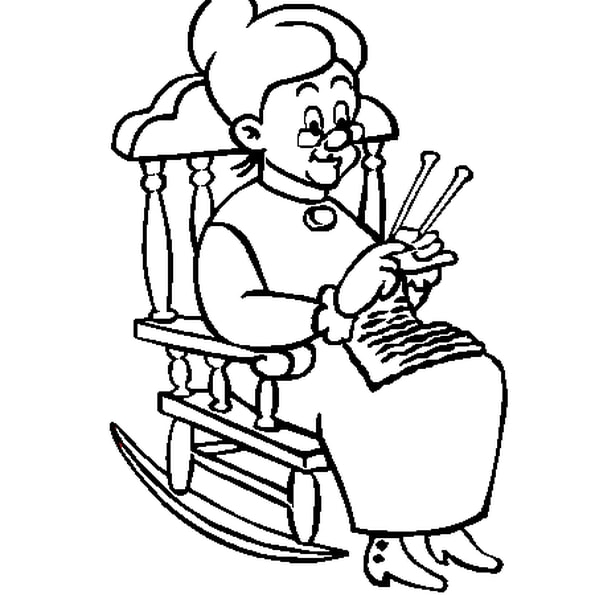
\includegraphics[width=0.4\textwidth]{daarwaseenwufdiespon}
\end{intersong}